\documentclass[a4paper,12pt]{article}
\usepackage[utf8]{inputenc} 
\usepackage[english]{babel}
\usepackage{graphicx} 
\usepackage{lmodern} 
\usepackage{cite}
\usepackage{hyperref}
\usepackage{listings}
\usepackage{color}
\usepackage{caption}
\usepackage{subcaption}
\usepackage[top = 3cm, left = 2.5cm, bottom = 2.5cm, right = 2.5cm]{geometry}
\hypersetup{pdfborder={0 0 0}}

% infos du document
\author{Jennifer Rondineau}
 
\begin{document}
 
\setlength{\parindent}{0cm}
\setlength{\parskip}{1ex plus 0.5ex minus 0.2ex}
\newcommand{\hsp}{\hspace{20pt}}
\newcommand{\HRule}{\rule{\linewidth}{0.5mm}}
\begin{titlepage}
  \begin{sffamily}
  \begin{center}

    
\includegraphics[scale=0.2]{logo.jpg}~\\[2cm]

    \textsc{\LARGE Université de Nantes}\\
    \textsc{\LARGE  }\\
    \textsc{\Large UFR Sciences et Techniques}\\
    \textsc{\LARGE  }\\
    \textsc{\LARGE  }\\
    \textsc{\Large Algorithmique et programmation avancées pour les biologistes}\\
    \textsc{\LARGE  }\\
    \textsc{\Large Algorithmes et méthodes pour la Bio-Informatique}\\[1cm]

    % Title
    \HRule \\[0.4cm]
    { \huge \bfseries Extraction de motifs communs à plusieurs séquences biologiques\\[0.4cm]
     }
    \HRule \\[2cm]

    % Author and supervisor
     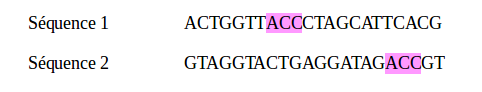
\includegraphics[scale=0.7]{deco.png}~\\[2cm]
    
 
      \begin{center} \large
       Ulysse \textsc{Guyet}\\
       Jennifer \textsc{Rondineau}\\
       Master 2 Bioinformatique \\
      \end{center}

    \vfill

    % Bottom of the page
    {\large 16 décembre 2015}

  \end{center}
  \end{sffamily}
\end{titlepage}
 % page de garde
\renewcommand{\contentsname}{Sommaire} 
\tableofcontents{} % afficher l'index
\clearpage
\lstset{language=bash, basicstyle=\small\ttfamily, breaklines,prebreak= , postbreak= , frame=shadowbox}

\section{Présentation du programme}

Le programme s'utilise en ligne de commande. Il prend en entrée plusieurs paramètres : 
\begin{enumerate}
\setlength{\itemsep}{1pt}
\setlength{\parskip}{0pt}
\setlength{\parsep}{0pt}
\item Un nom de fichier FASTA contenant les séquences à étudier
\item La longueur du motif commun à extraire
\item Le nombre maximal d'erreurs autorisées entre occurrence et motif (distance de Levenshtein)
\item Le quorum, le pourcentage minimum de séquences qui doivent présenter une occurrence du motif
\item Éventuellement un nom de fichier dans lequel l'utilisateur pourra sauvegarder les résultats de l'extraction
\end{enumerate}

\begin{lstlisting}
./extraction_motif -f seq.fa -d 1 -q 0.5 -s sauvegarde.txt
\end{lstlisting}

\vspace{1cm}
L'argument -h permet d'afficher une aide à l'utilisation du programme: \\
\vspace{0.2cm} \\
\fbox{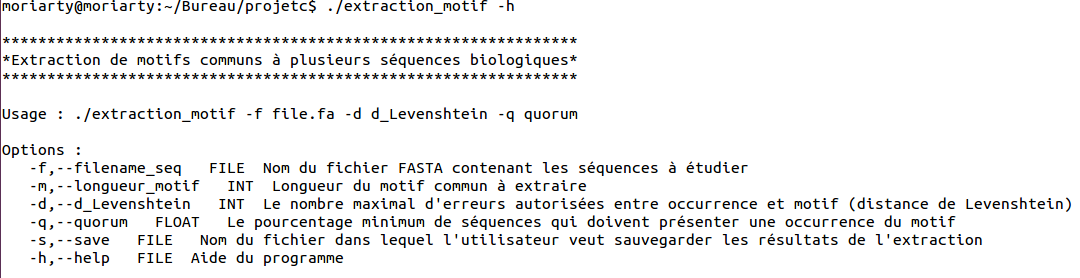
\includegraphics[scale=0.4]{help_screenshot.png}~}\\[1cm]
Après avoir entré les paramètres désirés à la suite du nom de l’exécutable, le menu suivant s'affiche:  \\
\vspace{0.2cm} \\
\fbox{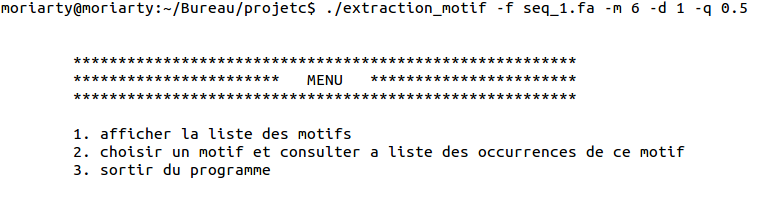
\includegraphics[scale=0.4]{menu_screenshot.png}~}\\

\subsection{Longueur du motif à extraire}

L'option "-m" définit la longueur du motif commun que l'on désire extraire des séquences, cette longueur est de type entier. Si cette longueur dépasse la longueur maximale des séquences, le dictionnaire est alors vide.  
\newpage
\subsection{La distance de Levenshtein}

La distance de Levenshtein correspond au nombre maximal d'erreurs autorisées entre l'occurrence et le motif, cette variable est de type entier, et on l'a définit avec l'option "-d", par défaut cette distance est de 0. Les erreurs peuvent correspondre à une insertion, une délétion ou une substitution. 

\subsection{Le quorum}

Le quorum correspond au pourcentage minimum de séquences qui doivent présenter une occurrence du motif. On définit cette variable par l'option "-q", elle est de type "float", et par défaut elle vaut 0. 

\subsection{La sauvegarde dans un fichier}

Si l'utilisateur donne en paramètre l'option "-s" suivit d'un nom de fichier pour la sauvegarde, le programme enregistre dans ce fichier les résultats de l'extraction des motifs communs (seulement après consultation d'un motif).

Exemple de ligne de commande : 
\begin{lstlisting}
./extraction_motif -f seq.fa -q 0.5 -s sauvegarde.txt
\end{lstlisting}

Le fichier "sauvegarde.txt" se présente ainsi : \\
\fbox{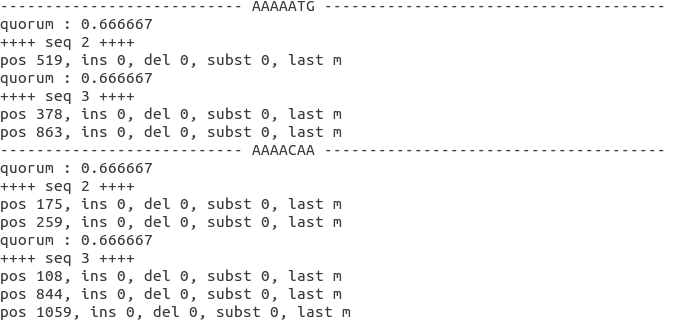
\includegraphics[scale=0.5]{sauvegarde.png}~}\\

Pour chaque motif, on sauvegarde le numéro de la séquence, la position, et les erreurs éventuelles (ins = insertion, del = délétion, subst = substitution, last = dernière opération réalisé (m = match, i = insertion, d = délétion, s = substitution). 
\newpage
\section{Les structures de données utilisées}
\begin{figure}[!h]
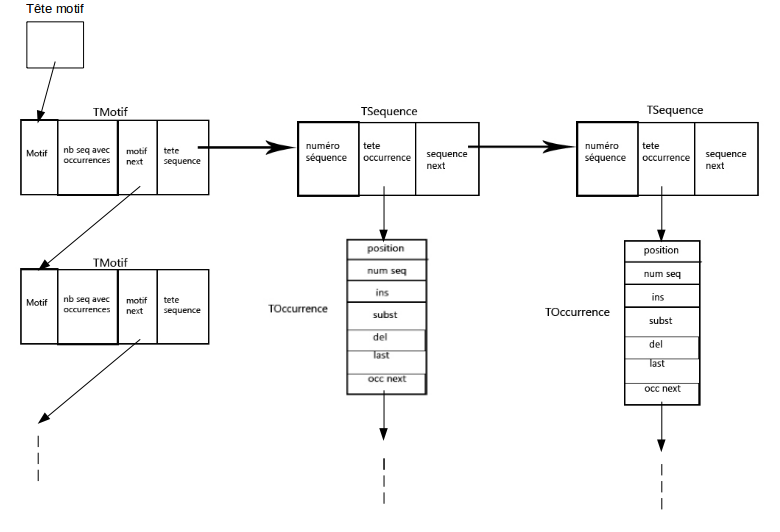
\includegraphics[scale=0.6]{structureDeDonnees.png}~
\caption{organisation des différentes structures}
\end{figure}
TeteMotif pointe vers une liste de motifs, qui pointe vers une liste de séquences et chaque séquence pointe vers une liste d'occurrences.

\section{Tests réalisés}

Nous avons d'abord effectué des tests sur des petites séquences, comme par exemple : 

\begin{lstlisting}
>Sequence1
AGGTCGATGCGGATGGCAGTTAA
>Sequence2
GGTAGATCTATAGGGCATTTA
\end{lstlisting}

Les figures ci-dessous montrent l'affichage de la liste des motifs (a) et le détail d'un motif en particulier (b).
\begin{figure}[h!]
\begin{subfigure}{.5\textwidth}
  \centering
  \fbox{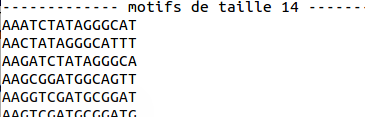
\includegraphics[scale=0.58]{affichage_liste_motifs.png}}
  \caption{aperçu de l'affichage de la liste des motifs}
  \label{fig:sfig1}
\end{subfigure}%
\begin{subfigure}{.5\textwidth}
  \centering
  \fbox{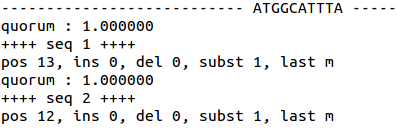
\includegraphics[scale=0.5]{affichage_details.png}}
  \caption{aperçu de l'affichage détail d'un motif}
  \label{fig:sfig2}
\end{subfigure}%
\end{figure}
Nous avons également comparé nos résultats d'extractions avec un autre binôme. A partir d'un même fichier FASTA et des mêmes paramètres de recherche (quorum, distance de Levenshtein, longueur du motif), nous avons retrouvé les mêmes résultats. 

\section{Les limites du programme} 

Si on désire réaliser une extraction de motifs communs à plusieurs séquences biologiques de taille importante, le temps de calcul devient assez conséquent. Plus les séquences sont longues, plus il faut du temps au programme pour extraire les motifs, surtout si on ajoute des erreurs possibles. 

Sans erreur, en définissant simplement la taille du motif et le quorum, le programme s’exécute relativement vite (moins d'une seconde pour 3 séquences d'environ 600 nucléotides chacune).

En revanche pour ces même séquences, si on accepte seulement deux erreurs possibles, le programme mettra environ 14 min à extraire les motifs communs. 

De même pour des séquences courtes : 

\begin{lstlisting}
>Sequence1
AGGTAGGAT
>Sequence2
AGGATTGA
\end{lstlisting}

Si on accepte 3 erreurs possibles sur un motif de longueur 7, et qu'on fixe le quorum à 50\%, le programme met 5 minutes à s'exécuter et on obtient 10 033 motifs possibles. 



\section{Améliorations à apporter au programme}

En ayant plus de temps, nous pourrions améliorer ce programme sur différents points : 
\begin{enumerate}
\setlength{\itemsep}{1pt}
\setlength{\parskip}{0pt}
\setlength{\parsep}{0pt}
\item L'enregistrement pourrait être amélioré, par exemple l'utilisateur pourrait enregistrer seulement les motifs qui l’intéresse. 

\item L'affichage des motifs pourrait également être amélioré. On pourrait imaginer un menu qui propose à l'utilisateur de visualiser toutes les occurrences de motifs présentant un délétion, une substitution ou un match. 

\item On pourrait rajouter des sécurités au niveau du getopt$\_$long, par exemple, faire quitter le programme si l'utilisateur indique une chaîne de caractère au lieu d'un entier pour la distance de Levenshtein. 

\end{enumerate}


\end{document} 